% !TEX program = arara-rc
% !TEX encoding = utf8
% !TEX spellcheck = en_GB
%:!arara settings
% arara: lualatex: { shell: true , synctex: true }
% !arara: lualatex: { shell: true , synctex: true }
%%: Start Header
\makeatletter
\RequirePackage{ifluatex}
\ifluatex
 \else
   \PackageError{xframed}{
    ^^J\space\space * This file requires LuaTeX.       
    ^^J\space\space * You  must change your typesetting engine                
  }
  \expandafter\endinput
\fi
\makeatother
\setcounter{errorcontextlines}{999}
\documentclass[openany,12pt,tocdepth=3]{ltx-md}

\usepackage{frcursive}
\usetikzlibrary{decorations.pathmorphing}
\RequirePackage{minted}
\usemintedstyle{autumn}
\fvset{xleftmargin=0.2cm,xrightmargin=.2cm}
\renewcommand*{\dictumwidth}{.5\textwidth}
\setcounter{secnumdepth}{3}

\ExplSyntaxOn
\keys_define:nn {ltxexample}
 {
  caption  .tl_set:N = \l_mdxex_caption_tl,
  label    .tl_set:N = \l_mdxex_label_tl,
  minted   .tl_set:N = \l_mdxex_minted_tl,
  minted   .initial:n = {linenos=true} ,
  language .tl_set:N = \l_mdxex_language_tl,
  language .initial:n = latex,
  result   .bool_set:N = \l_mdxex_result_bool,
  result   .initial:n =false,
}

\NewDocumentEnvironment {ltxexample} { O {} }
 {
  \keys_set:nn { ltxexample }
   {
    #1
   }
  \group_begin:
  \tl_set:Nx \l__mdxex_temp_tl
   {
    \exp_not:N \VerbatimEnvironment
    \tl_if_empty:NTF \l_mdxex_caption_tl
     {
      \scan_stop:
     }
     {
      \exp_not:N \xframedsetup 
          {
             line-color=brown!70!black,
             bg-color=brown!10!white,
             inner-top-margin=12pt,
             inner-bottom-margin=0pt,
             title-above-skip = 6pt,title-below-skip=6pt,
             title-bg-color = brown!15!white,
             line-width-top=2pt,margin=1cm,
             first-title= { \exp_not:N \captionof { lstlisting }{ \exp_not:V \l_mdxex_caption_tl } 
                                \tl_if_empty:NF \l_mdxex_label_tl
                                 { \exp_not:N \label { lst\exp_not:N : \l_mdxex_label_tl } }
                               } 
         }
     }
    \exp_not:n { \begin{xframed}[]\begin{minted} } [ \l_mdxex_minted_tl ] { \l_mdxex_language_tl }
   }
  \l__mdxex_temp_tl
 }
 {\end{minted}\end{xframed}%
  \group_end:\bool_if:NT \l_mdxex_result_bool { \input{\jobname.pyg} }
}
%%%\NewDocumentEnvironment {ltxexample} { sO {} }
%%% {
%%%  \keys_set:nn { ltxexample }
%%%   {
%%%    #2
%%%   }
%%%  \tl_set:Nx \l__mdxex_temp_tl
%%%   {
%%%    \exp_not:N \VerbatimEnvironment
%%%    \tl_if_empty:NTF \l_mdxex_caption_tl
%%%     {
%%%      \scan_stop:
%%%     }
%%%     {
%%%      \exp_not:N \xframedsetup 
%%%          {
%%%             line-color=brown!70!black,
%%%             bg-color=brown!10!white,
%%%             inner-top-margin=0pt,
%%%             inner-bottom-margin=0pt,
%%%             title-above-skip = 6pt,title-below-skip=6pt,
%%%             title-bg-color = brown!15!white,
%%%             line-width-top=2pt,margin=1cm,
%%%             first-title= { \exp_not:N \captionof { lstlisting }{ \exp_not:V \l_mdxex_caption_tl } 
%%%                                \tl_if_empty:NF \l_mdxex_label_tl
%%%                                 { \exp_not:N \label { lst\exp_not:N : \l_mdxex_label_tl } }
%%%                               } 
%%%         }
%%%     }
%%%    \exp_not:n { \begin{xframed}[]\begin{minted} } [ \l_mdxex_minted_tl ] { \l_mdxex_language_tl }
%%%   }
%%%  \l__mdxex_temp_tl
%%% }
%%% {\end{minted}\end{xframed}}
\RenewDocumentCommand\DeleteFile{m}{}
%\NewDocumentCommand\NotDeleteFile{}{%
%    \DeleteFile {\jobname.pyg}%
%    \DeleteFile {\jobname-out.pyg}%
%    \RenewDocumentCommand\DeleteFile{m}{}
%}\input{\jobname.pyg}
\ExplSyntaxOff
\NewDocumentCommand \Github {} {Github\faGithub\xspace }
\usepackage{xframed}
\begin{document}
\title{The \Pack{xframed} package}
\subtitle{This is an alpha-version}
\author{Marco Daniel}
\date{\today}
\notes{As shown in the subtitle this is an alpha version. Use this package on your own
risk.\\[.5cm]
I know my English is really poor and the quality of the documentation suffers on it. 
So I am really happy about any improvments.\\[1cm]

As long as the package has the version alpha I am not deprecated to change names
of options. My aim is to use as many intuitive options as possible. 
}
\maketitle
\vspace*{\fill}
\begin{xframed}[line-width=3pt,line-color=purple!30!white,bg-color=yellow!10,developer-info,margin=1cm]
\rule{0pt}{5cm}
\end{xframed}
\clearpage
\pdfbookmark[1]{\contentsname}{tocbook}
\tableofcontents


\setchapterpreamble[o]{\dictum[\href{http://tex.stackexchange.com/a/18360/5239}{Gonzalo Medina at TeX.SX}]{%
Expand $(a+b)^n$:
\begin{center}
  \count255=0
  \loop\advance\count255 by 10
  \ifnum\count255<40
    $(a\hskip\count255 pt +\hskip\count255 pt b)^n$\\
  \repeat
\end{center}}}
\addchap{Preface}
\addsec{Introduction}\label{sec:intro}
I am interested in \LaTeX\ and specially in \LaTeX3. With this package I want
to improve my skills using this great language. However I am a beginner and
so the package has only an \textit{alpha} version. If you use this package
be aware of this situation. I am sure the great guys at
\faArrowRight\href{http://tex.stackexchange.com/}{TeX.SX} will help me to improve this package.


\addsec{Bug reports}\label{sec:bug-reports}
Bug reports can be done at
\href{https://github.com/marcodaniel/xframed/issues}{xframed at \Github}. If you have no
account at \Github you can drop me an e-mail
\href{mailto:marco.daniel@mada-nada.de}{\faEnvelope marco.daniel@mada-nada.de}

\addsec{Installation}
As long as the package isn't available at CTAN you must install (if you dare it)
manual. Therefor you can clone the repository in your local texmf tree. I provided
the correct folder structure at \Github to simplify the installation.

\setchapterpreamble[o]{\dictum[]{%
If you are only interested in the usage of the package you can
skip this chapter. All options are explain in \autoref{chap:usage}}}
\chapter{Idea behind \texorpdfstring{\Pack{xframed}}{xframed}}\label{chap:idea}

The idea is very simple. Draw a frame around given material. During my study 
I wanted a package which can be break across pages and put a frame around this.
The package \Pack{framed}\footnote{Package \Pack{framed} by Don­ald Arse­neau, 
see \href{http://www.ctan.org/pkg/framed}{CTAN: framed}} didn't require my needs.
So I started to write my own package. The result can be found at CTAN, too. It's the
package \Pack{mdframed}\footnote{Package \Pack{mdframed} by Marco Daniel, 
see \href{http://www.ctan.org/pkg/mdframed}{CTAN: mdframed}}.

After passing my study I started to improve the package \Pack{mdframed}. In 2011 
I registered at \href{http://tex.stackexchange.com/}{TeX.SX}  and learned something
about the new language \Pack{expl3}\footnote{see: 
\href{http://latex-project.org/latex3.html}{http://latex-project.org/latex3.html}}. 
I was so fascinated about the great work of the \LaTeX3 core team that I started 
my first steps with simple functions. I also wrote a small article about the 
frontend \Pack{xparse} for the German community. The article was published
in   \emph{Die \TeX nische Komödie 2/2012}. 
After a while I wanted to provide my own \Pack{expl3}-package. Now here it is.

I know most users love examples. So I am trying to provide a lot. All
frames in this documentation are done by \Env{xframed}. So I hope
you will have some inspiration. The higlight of listings is done
by \Pack{minted}\footnote{Package \Pack{minted} by Kon­rad Ru­dolph, 
see \href{http://www.ctan.org/pkg/minted}{CTAN: minted}, now maintained by G. Poore.}.

\vfill
By the way. The compiliation of this document is done with the
typesetting enginge \LuaLaTeX. To simplify my compilation steps
I am using the cool tool \Pack{arara}\footnote{Tool \Pack{arara} by Paulo Cereda, 
see \href{http://www.ctan.org/pkg/arara}{CTAN: arara}}.

\vfill
Now it's time to introduce the package.


\setchapterpreamble[o]{\dictum[\href{http://tex.stackexchange.com/a/18370/5239}{Jaime Soto at TeX.SX}]{%
\begin{eqnarray*}
    \begin{bmatrix}
    \cos 90^{\circ} & \sin 90^{\circ}\\
   -\sin 90^{\circ} & \cos 90^{\circ}
\end{bmatrix}
\begin{bmatrix} a1 \\ a2 \end{bmatrix}
=
\rotatebox[origin=c]{270}{$\begin{bmatrix} a1 \\ a2 \end{bmatrix}$}
\end{eqnarray*}}}
\chapter{Usage}\label{chap:usage}
The following sections descripe the options of the package and the provided 
environments. The basic environment is equal to the package name \Env{xframed}.

\section{Loading the package}
Before you can use the package, you must load it in your preamble. As usual the 
package is loaded by \Cmd{usepackage}. The following listings shows it.
\begin{ltxexample}[caption=Loading the package,label=loading]
 % Preamble
 \usepackage{xframed}
\end{ltxexample}
If you have done this you can use the basic environment \Env{xframed}.

\ExplEnv{xframed}
The environment has one optional argument where you can specify options
which are only used for this frame. The following listings demonstrates the usage.
\begin{ltxexample}[caption=Loading the package,label=loading]
 % document body
 \begin{xframed}[option-list]
   The contents of the frame
 \end{xframed}
\end{ltxexample}

\section{Specifying the options}
Before you setup any options you must understand hot the frame is drawn.
The default method is by using \Pack{TikZ}\footnote{Package \Pack{TikZ} by 
Till Tantau \& friends, see \href{http://www.ctan.org/pkg/pgf}{CTAN: TikZ}}. 
\Pack{TikZ} allows a very user friendly way to setup high quality graphics. 
Therefor all elements are specified by \Pack{TikZ} options. The basic command
to manipulate these elements is \Cmd{xframedsetuptikz}. The usage is explained
in \autoref{se:tikzsetup}.  All other options can be set by \Cmd{xframedsetup}. 
Both command can be used in the preamble or inside the document body. If
you enclose these commands inside a group the settings will be local, too.
 
\ExplCmd{xframedsetuptikz\MArgs}
The command has one mandatory argument. The mandatory argument accepts only
defined options which are explaind in \autoref{se:tikzsetup}

All other options can be setup by the command \Cmd{xframedsetup}.
\ExplCmd{xframedsetup\MArgs}
This command has one mandatory argument. All allowed options are explained
in \autoref{chap:options}. 

\section{Helper functions}\label{sec:helperfunctions}
The next function will normally be used by advanced users. However
I decided to put this information here instead of in
\autoref{chap:developer-info}~\nameref{chap:developer-info}.
All commands have one mandatory argument. The mandatory argument
is one of the explained keys in the following sections. Please note 
that the argument doesn't accept a meta key.

\ExplCmd{usexframendlength}[\MArgs[key]]
This command  allows you to use the
provided length inside an other command. The \texttt{key} is one of
the length keys explained in the following sections. 
\ExplCmd{showxframendlength}[\MArgs[key]]
The command \Cmd{showxframendlength} has one important
difference to \Cmd{usexframendlength}. The provided length
can be printed inside the document. For you my \TeX-hacker
that means the primitive \Cmd{the} is used. 

\ExplCmd{usexframendskip}[\MArgs[key]]
This command is equal to \Cmd{usexframendlength} whereby
a skip key is required.
\ExplCmd{showxframendskip}[\MArgs[key]]
I think you know what happen here. See \Cmd{showxframendlength}, 
it's only for skip length.
\ExplCmd{usexframendcolor}[\MArgs[key]]
This command is similar to the command \Cmd{color}, whereby the
color of the provided option is used.
\ExplCmd{showxframendcolor}[\MArgs[key]]
This command print out the color which is hidden under the key.

\minisec{Example}
Next to the explanation I want to provide an example. 

\begin{ltxexample}[caption=Example of helper functions,label=helper,result=false,]
 \begin{xframed}
    \showxframendskip{ski-above}%
    \hspace{\usexframendlength{inner-left-margin}}%
    \showxframendcolor{fon-color}
 \end{xframed}
\end{ltxexample}


\section{Creating new environments}\label{sec:newenv}

\ExplCmd{Newxframedenv}[\OArgs\MArgs[env-name]]
\ExplCmd{Renewxframedenv}[\OArgs[env-name]]
\ExplCmd{Surroundwithxframed}[\OArgs\MArgs[env-name]]






Before we start with options we need to understand the provided elements of the frame. 

\section{Elements of the frame drawn by \texorpdfstring{\Pack{xframed}}{xframed}}
It should be clear the a frame has some rules around. So we can check mark the first
relevant point.The next point of the agende is the main body, the title and the foot. These
three elements are very important to understand the behaviour. The simple picture below
should show the elements and the provided names inside the package.

\begin{center}
\captionof{figure}{Base elements of \texorpdfstring{\Pack{xframed}}{xframed}}\label{fig:baseelements}
\begin{tikzpicture}[outer sep=0pt]
 \node[draw,rectangle,minimum width=8cm, minimum height=2cm,font=\bfseries] (main) {Body of the frame~\faArrowRight~\texttt{main}};
 \node[draw,rectangle,minimum width=8cm, minimum height=1cm,font=\bfseries,anchor=south] at (main.north) {Title of the frame~\faArrowRight~\texttt{first-title}};
 \node[draw,rectangle,minimum width=8cm, minimum height=1cm,font=\bfseries,anchor=north] at (main.south) {Foot of the frame~\faArrowRight~\texttt{last-foot}};
\end{tikzpicture}
\end{center}
I know the picture looks very poor at the beginning but we want to concentrate on the
main issue. It descripes the three base elements of the frame drawn by \Env{xframed}.

\vspace*{\baselineskip}
Now let's start with all options. Be aware the list ist long. 

\setchapterpreamble[o]{\dictum[\href{http://tex.stackexchange.com/a/18354/5239}{Paulo Cereda at TeX.SX}]{%
Find $x$.

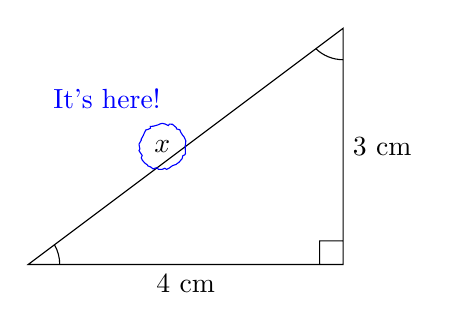
\begin{tikzpicture}
\draw (0,0) -- (4,0) node[midway,below] {4 cm}
   -- (4,3) node[midway,right] {3 cm}
   -- (0,0) node[midway,left,circle,draw=blue,decorate,decoration={random steps,segment length=1pt,amplitude=0.5pt}]{$x$}
   -- (4,0) rectangle (3.7,0.3)
   -- cycle;
\draw (0.4,0) arc (0:30:0.5);
\draw (4,2.6) arc (270:226:0.5);
\draw (1,2.1) node []{\color{blue}\fontfamily{frc}\selectfont{It's here!}};
\end{tikzpicture}}}

\chapter{Package options}\label{chap:options}
Every user has his/her own wishes. It's very difficult to implement an evironment 
which meets all requirements. I hope with the following options you can setup your 
requirements as best as I was able to implement. As described in \autoref{chap:idea}
the package uses \Pack{expl3} in the background. So I can provide more intuitive names.
During the explanation I refer to the environment \Env{framed}. However this is only
symbolic. The options are also working for other derivations. 

\section{Outside the frame}
Drawing a frame requires some modifcations around. So you want to setup the margins
or the skips above or below the frame. Related to the meaning of the keys, all keys 
requiers a length or skip dimension. That mean that the length variables defined as
\texttt{dim} have a fixed length, whereas \texttt{skip} length can have a rupper (stretch/shrink) component. 

\ExplOpt{width}

\ExplOpt{minimum-space}

\ExplOpt{skip}
This is the length represented the space before and after the environment \Env{xframed}.  
This options is a meta key and sets the \Opt{skip-below} and \Opt{skip-above} to the given skip length. 
\ExplOpt[10pt]{skip-above}
As described at \Opt{skip} this skip length specify the space above the frame.
\ExplOpt[10pt]{skip-below}
Related to the other options here you can setup the space after the environment.


\ExplOpt{margin}
Normally the frame \Env{xframed} is drawn about the complete text width. However this isn't
often very common. This keys accept a dimension length which specify the left and the right margin.
You can also use negativ values. In this case the frame is drawn inside the margin of the page.
\ExplOpt[0\,pt]{left-margin}
Here you can setup the left margin separat. 
\ExplOpt[0\,pt]{right-margin}
And here the right margin. 

\ExplOpt[0\,pt]{extra-skip}
Sometimes it's useful to add some vertical white space in front of the frame. This can be useful
if you want some elements on the lines. To take care of this required space you can
set the Option \Opt{extra-skip}. Negative dimensions are also allowed whereby I can't
image any situation to use it. 
\ExplOpt{top-line}%bool-option
\ExplOpt{left-line}%bool-option
\ExplOpt{bottom-line}%bool-option
\ExplOpt{right-line}%bool-option

\ExplOpt{round-corner}%metakeys
\ExplOpt{arc}%metakeys
\ExplOpt{outer-arc}

\vspace*{\baselineskip}
This finished the \emph{outside} part for the moment. The package provides also some hooks
which will can be used as an option. This isn't really a low level issue so these
options are desribed in \autoref{sec:hook}. 

\vspace*{\baselineskip}
Before I will descripe the options related to there base element as shown in \autoref{fig:baseelements}, 
I will start with the rules around the frame.

\section{Rules around the frame}\label{sec:lines}
A normal frame has four sides. The frame of \Env{xframed} isn't an exception. Of course
you can manipulate as possible to get a triangle or a star.

\ExplOpt{line-width}
The first option in this section specify the width of all four lines around the material of \Env{xframed}.
This implices the title and the foot of the frame. If you want to setupt the rule width of the elements
separate you can do this by the following options.
\ExplOpt[0.8\,pt]{line-width-left}
Specifies the width of the left line.
\ExplOpt[0.8\,pt]{line-width-right}
Specifies the width of the right line.
\ExplOpt[0.8\,pt]{line-width-top}
Specifies the width of the top line.
\ExplOpt[0.8\,pt]{line-width-bottom}
Specifies the width of the bottom line.

The width is only one part of the lines. I am sure you want to change the colors too. 
\ExplOpt{line-color}
Normally all lines have the same color. The color for all four lines can be specified 
with the Option \Opt{line-color}. However the following keys allow the color
specification separat.
\ExplOpt[black]{line-color-right}
Specifies the color of the right line.
\ExplOpt[black]{line-color-top}
Specifies the color of the top line.
\ExplOpt[black]{line-color-bottom}
Specifies the color of the bottom line.

\ExplOpt{inner-arc}

\minisec{Example}
I think it's time for a small example. Suppose you want that all lines has a width of
2\,pt expect the top line which shall have a width of 4pt and a different color.
This can be achived by
\begin{ltxexample}[caption=Example outer part,label=outer,result=true,]
 \begin{xframed}[line-width=2pt,line-width-top=4pt,
          line-color-top=blue]
   The contents of the frame
 \end{xframed}
\end{ltxexample}
As a small revision we can achive the same effect with \Cmd{xframedsetup}, 
whereby the settings are used for the the environemnts \Env{xframed} to follow.
\begin{ltxexample}[caption={Example outer part II},]
 \xframedsetup[line-width=2pt,line-width-top=4pt
           ,line-color-top=blue]
 \begin{xframed}
   The contents of the frame
 \end{xframed}
\end{ltxexample}

As you can see the topline gets a smooth transition. 

\ExplOpt{show-all-lines}%metakeys

\section{Main body of the frame}\label{sec:element-main}
As shown in \autoref{fig:baseelements} the body is the main part of
the environment \Env{xframed}. Inside the body you can use every
material also verbatim one. This part is save in a single coffin%
\footnote{See: \Pack{l3coffin}}  and allows such things. 

\ExplOpt[\string\normalfont]{font}
The option \Opt{font} allows the specification of the main part of \Env{xframed}.
It doesn't influence the other part. 

\ExplOpt[black]{font-color}
If you want to change the font color you can do this with the option \Opt{font-color}.

\ExplOpt[white]{bg-color}
The complete background of \Env{xframed} is specifed by the color given
as an argument of \Opt{bg-color}. If you want some shadings or whatever
you can imagine you can the power of tikz. How to do this
is explained in \autoref{sec:tikzsetup}.

\ExplOpt[10\,pt]{inner-margin}
The distance on the left site and the right site of the frame will be 
controled by \Opt{inner-left-margin} and \Opt{inner-right-margin}. The 
key \Opt{inner-margin} sets the relevant lengths. However you can 
setup left and right alone.
\ExplOpt[10\,pt]{inner-left-margin}
Specifies the left margin of the frame.
\ExplOpt[10\,pt]{inner-right-margin}
Specifies the right margin of the frame.

\faArrowRight Please note: the length will be used for the other two elements as shown in 
\autoref{fig:baseelements}, too.

 Related to the left and right margin you can set the top and bottom margin.
\ExplOpt{inner-top-margin}
This keys sets the top margin of the main part.
\ExplOpt{inner-bottom-margin}
This keys sets the bottom margin of the main part.


\minisec{Head of the frame}
Sometimes you want to have a small head without any brek. This
can be achieved by the key \Opt{head}. I implement this key with 
some other options to simplify e.g. the creating of a new thereom. There
is also another option \Opt{first-title} which is used in a new coffin and
so put in an extra box. At the momemnt all cpations of the provided linstings
are done in the \Opt{first-title}. 


\ExplOpt{head}
Puts the given argument of \Opt{head} at the beginning
of the main body.
\ExplOpt[\string\normalfont\string\sffamily\string\bfseries]{head-font}
The font is specified by the option \Opt{head-font} which be set set local as
also the color.
\ExplOpt[black]{head-font-color}
Specifies the color of the head.


\minisec{Head of the frame}
I guess at this point an example is useful. Instead of explaining I 
only provide the example.

\begin{ltxexample}[caption={Example main part},label=main,result=true]
 \begin{xframed}[%
   line-width=4pt,line-color=blue,
   inner-margin=1cm,font-color=blue!70,
   head={Example of Head},head-font-color={red!70},
   margin=1.5cm,bg-color=yellow!20,
  ]
   The contents of the frame and some filling text to 
  provide a second line.
 \end{xframed}
\end{ltxexample}


\section{Title of the frame}\label{sec:element-firsttitle}
The title of the frame is specied by an option and also save in a coffin. 
This means the paragraphs of the body can't be influence by material
of the title. Here you can see the first main differences between
\Opt{first-title} and \Opt{head}. Let us start with options.

\ExplOpt{first-title}
First of all we need a title. The title can be specified by \Opt{first-title}. The argument
is saved in a single token. Of course you can use line breaks but please encapsule
the whole argument in curly braces. Curly braces must be used if you argument contains
a comma. May you wonder why it's named \Opt{first-title}. If the frame
must be splitted the \Opt{first-title} is only used at the first frame. If
you don't have any splitted frame, you have only one tile the \Opt{first-title}.
\ExplOpt[\string\bfseries\string\sffamily\string\large]{title-font}
Normally the title should be highlighted. So I decided to declare the list of
font commands as default. However you can use the option \Opt{title-font} to
declare your own font setttings.
\ExplOpt[black]{title-font-color}
As usual you can specify the color of the font. This is done by the option
\Opt{title-font-color}.

\ExplOpt[5pt]{title-skip}
As written the title is put inside a new coffin. The explained options \Opt{inner-margin},
\Opt{inner-left-margin} and \Opt{inner-right-margin} will be used on the left and right side of
the title component. However you can specify the length above and below the contents of the title. 
The option \Opt{title-skip} passes the argument to the options \Opt{title-above-skip}
and \Opt{title-below-skip}.
\ExplOpt[5pt]{title-above-skip}
Specify the length betweend the top line and the material of \Opt{first-title}.
\ExplOpt[5pt]{title-below-skip}
Specify the length betweend the new line \Opt{title-line} and the material of \Opt{first-title}.

\faArrowRight Please note:  I know the name \texttt{skip} leads to irritations. The length are save in a
dimension register and so any glue will be cut.

\ExplOpt[white]{title-bg-color}
As the main part you can specify a different color as background for
the title. This color of the option \Opt{title-bg-color} will be used for it.


The package \Pack{xframed} provides a single line between the title and the main body.
The following options show you the usage. Of course with methods of
\autoref{sec:tikzsetup} you can draw dashed lines or other one as well.
\ExplOpt[true]{title-line}
The option \Opt{title-line} is a bool key. If you say \texttt{true} a line to separat
the material will be drawn. If you say \texttt{false}, you will get no line.
\ExplOpt[0.6pt]{line-width-title}
The width of the line is specified by the option \Opt{line-width-title} whereby
the width doesn't influence the length \Opt{inner-top-margin} and \Opt{title-below-skip}.
\ExplOpt[black]{title-line-color}
Last but not least the color of the line is done by \Opt{title-line-color}.

\minisec{Example}
It's time for a new example to demonstrate the title.

\begin{ltxexample}[caption={Example title part},label=title,result=true]
 \begin{xframed}[title-bg-color=brown!30,%
   line-width=2pt,line-color=brown!60,
  first-title={This is the title of the frame},
   margin=1.5cm,bg-color=yellow!20, ]
   The contents of the frame and some filling text to 
  provide a second line.
 \end{xframed}
\end{ltxexample}



\section{Foot of the frame}\label{sec:element-lastfoot}
The settings of the foot element are equal to the title element. So 
the explanation will be short. 
\ExplOpt{last-foot}
The foot can be specifed by \Opt{last-foot}. Of course now you
know why it is named \Opt{last-foot} (related to \Opt{first-title},
\ExplOpt[\string\bfseries\string\sffamily\string\small]{foot-font}
The foot is normally a little bit smaller so I decided to use \Cmd{small} as
default.


\ExplOpt[black]{foot-font-color}
Specify the color of the font.

\ExplOpt[5pt]{foot-skip}
The option \Opt{foot-skip} passes the argument to the options \Opt{foot-above-skip}
and \Opt{foot-below-skip}.
\ExplOpt[5pt]{foot-above-skip}
Specify the length betweend the separation line between the main part and the material of \Opt{last-foot}.
\ExplOpt[5pt]{foot-below-skip}
Specify the length betweend the frame and the material of \Opt{last-foot}.

\faArrowRight Please note:  I know the name \texttt{skip} leads to irritations. The length are save in a
dimension register and so any glue will be cut.

\ExplOpt[white]{foot-bg-color}
As the main part you can specify a different color as background for
the foot. This color of the option \Opt{title-bg-color} will be used for it.


The package \Pack{xframed} provides a single line between the foot and the main body.
The following options show you the usage. Of course with methods of
\autoref{sec:tikzsetup} you can draw dashed lines or other one as well.
\ExplOpt[true]{foot-line}
The option \Opt{foot-line} is a bool key. If you say \texttt{true} a line to separat
the material will be drawn. If you say \texttt{false}, you will get no line.
\ExplOpt[0.6pt]{line-width-foot}
The width of the line is specified by the option \Opt{line-width-foot}.
\ExplOpt[black]{foot-line-color}
Last but not least the color of the line is done by \Opt{foot-line-color}.


\minisec{Example}
It's time for a new example to demonstrate the title.

\begin{ltxexample}[caption={Example foot part},label=foot,result=true]
 \begin{xframed}[title-bg-color=brown!30,%
   foot-bg-color=brown!30,line-width=2pt,
   line-color=brown!60,margin=1.5cm,bg-color=yellow!20, 
   first-title={This is the title of the frame},
   last-foot={you reached the end},]
   The contents of the frame and some filling text to 
  provide a second line.
 \end{xframed}
\end{ltxexample}


\section{Tikz elements of  \texorpdfstring{\Pack{xframed}}{xframed}}\label{sec:tikzsetup}
Text 
\ExplOpt{setup-tikz}%hooks--tl


\section{Footnotes}\label{sec:footnotes}
\ExplOpt{footnote-distance}%skip keys
\ExplOpt{footnote-line-width}
\ExplOpt{footnote-line-lenght}
\ExplOpt{footnote-inside}%bool-option

\section{Subtitle(s)}\label{sec:subtitle}
\ExplOpt{subtitle-above-skip}
\ExplOpt{subtitle-below-skip}
\ExplOpt{subsubtitle-above-sk}
\ExplOpt{subsubtitle-below-sk}
\ExplOpt{subtitle-above-skip}%skip keys
\ExplOpt{subtitle-below-skip}%skip keys
\ExplOpt{subsubtitle-above-skip}%skip keys
\ExplOpt{subsubtitle-below-skip}%skip keys
\ExplOpt{subtitle-font-color}%colorkeys
\ExplOpt{subtitle-line-color}%colorkeys
\ExplOpt{subtitle-bg-color}%colorkeys
\ExplOpt{subsubtitle-font-color}%colorkeys
\ExplOpt{subsubtitle-line-color}%colorkeys
\ExplOpt{subsubtitle-bg-color}%colorkeys
\ExplOpt{shadow-color}%colorkeys
\ExplOpt{subtitle-font}%fontoptions--tl
\ExplOpt{subsubtitle-font}%fontoptions--tl
\ExplOpt{subtitle-line}%bool-option
\ExplOpt{subsubtitle-line}%bool-option

\section{shadow}\label{sec:shadow}
\ExplOpt{shadow-size}
\ExplOpt{shadow}%bool-option

\section{Hooks}\label{sec:hook}
Text 
\ExplOpt{code-before}%hooks--tl
\ExplOpt{code-after}%hooks--tl
\ExplOpt{subtitle-before}%hooks--tl
\ExplOpt{subtitle-after}%hooks--tl
\ExplOpt{subsubtitle-before}%hooks--tl
\ExplOpt{subsubtitle-after}%hooks--tl
\ExplOpt{code-single-frame}%hooks--tl
\ExplOpt{code-first-frame}%hooks--tl
\ExplOpt{code-middle-frame}%hooks--tl
\ExplOpt{code-last-frame}%hooks--tl
\ExplOpt{user-settings}%hooks--tl
\ExplOpt{post-tikz-code}%hooks--tl
\ExplOpt{first-tikz-code}%hooks--tl
\ExplOpt{middle-tikz-code}%hooks--tl
\ExplOpt{last-tikz-code}%hooks--tl
\ExplOpt{head-pre-code}%hooks--tl
\ExplOpt{head-post-code}%hooks--tl
\ExplOpt{head-post-code}%hooks--tl
\ExplOpt{title-pre-code}%hooks--tl
\ExplOpt{title-post-code}%hooks--tl
\ExplOpt{foot-pre-code}%hooks--tl
\ExplOpt{foot-post-code}%hooks--tl

\section{Important typographical notes}
\ExplOpt{ignore-last-descender}%bool-option
\ExplOpt{ignore-last-skip}%bool-option

\chapter{Breaking across pages}\label{chap:break}
Text 
\ExplOpt{allow-breaking}%bool-option
\ExplOpt{split-topskip}%skip keys
\ExplOpt{split-bottomskip}%skip keys
\ExplOpt{repeat-title}%bool-option
\ExplOpt{first-title}%stringoptions
\ExplOpt{last-foot}%stringoptions

\chapter{Developer Info}\label{chap:developer-info}

Text 
\ExplOpt{developer-info}%bool-option
\chapter{Examples}\label{chap:examples}
Text 

\appendix
\chapter{Appendix}\label{chap:appendix}
\section{Thanks}
Text 
\section{Bugs}
Text 

\section{ToDo}
\ExplOpt{twoside-mode}%bool-option
\end{document}
